\section{Theory and Hypotheses}

\subsection{Introduction and Prior Research}

There are several reasons why firms initiate open source (OS) projects. As \cite{west2003open} noticed, firms do publish source code in order to get their product widely adopted, to increase the likelihood to attract developers \footnote{first-mover advantages} and to achieve faster technological development (\cite{lerner2002some}). Beside that, all OS projects can be termed as collective action model which applies to the provision of public goods, where a public good is non-excludable and non-rival \cite[p.14]{olson2009logic}. Thus, OS projects can be regarded as foundation for a novel, private-collective model for the motivation of innovation (\cite{hippel2003open}). This confirms the assumption that any interested person can voice their opinion when organizations search for innovation by soliciting suggestions from externals (\cite{alexy2012managing}). Most OS projects which are initiated by firms are also part of their business. Hence, they utilize resources as knowledge and ideas to maximize their value creation and profit in the long run (\cite{dahlander2005relationships}).

Because OS projects of firms depend on the symbiotic relationship between internal end external developers, externals' suggestions can lead organizations to novel, useful, and actionable ideas (\cite{hill2009idea}), develop new concepts (\cite{katila2002something}; \cite{jeppesen2010marginality}; \cite{shane2000prior}) or find new markets for their technologies (\cite{gruber2008look}; \cite{shane2000prior}). So the "wisdom of the crowds" (\cite{surowiecki2005wisdom}) depends on external suggestions which facilitates research on external sources of innovation (\cite{dahlander2005relationships}) as on open innovation (\cite{chesbrough2003logic}), crowdsourcing (\cite{afuah2012crowdsourcing}) and user-based innovation (\cite{von1986lead}).

Most initiatives to engage external contributors do fail as \cite{dahlander2014open} showed in their study. They developed arguments about what increases the likelihood of getting suggestions from externals by proactive and reactive attention to suggestions. They say that firms and communities have divergent rationales for existing which causes problems on interaction. Moreover, they found out that early organizations' engagements weigh more in the early stage and that firms should pay attention to new contributors. Thus, they suggest to keep entry barriers low since it results in a lower threshold for participation.

\cite{piezunka2013study} developed a theory about the structures that are build around a suggestion after it is posted. They say the more suggestions are related to each other, the greater is the demand of externals for a suggestion. Additionally, the more a suggestion is debated by externals, the higher the likelihood an organization will attend to it. On the other side, the greater the diversity of suggestions and the more suggestions competes with each other, the lower the likelihood that an organization will attend to it.

One of the initial ideas of the OSS community is to work for non-commercial reasons. This means that firms have to deal with the term openness (\cite{dahlander2010open}) and have to accept that external developers are free to join and work on informal relationships (\cite{dahlander2005relationships}) whereas firm-based software creation is normally restricted to relations within the firm. To use the taxonomy by \cite{feller2002understanding}, we can distinguish between economic, social and technological motivation factors. As \cite{bonaccorsi2006comparing} found out, firms are driven by economic and technological factors rather than by social motivation factors. Contribution of external developers depends on both extrinsic and intrinsic motivation \footnote{which is a social motivation} (\cite{hertel2003motivation}; \cite{hars2001working}; \cite{lakhani2002boston}) or even by intellectual challenges (\cite{raymond2001cathedral}; \cite{hertel2003motivation}). This supports the assumption that users often find solutions to their own problems and are willing to share them when the marginal cost of sharing is low (\cite{von1976dominant}). Furthermore, users in OS projects are not protected by intellectual property rights (\cite{waguespack2004penguins}), which is converse to intellectual property handling of traditional (in-house) software development by firms.

\cite{west2008role} analyzed how corporate sponsorship influences OS communities. They identified three design dimensions for corporate sponsorship when designing OS communities:

\begin{enumerate}
	\item intellectual property rights
	\item development approach, and
	\item model of community governance
\end{enumerate}

Overall they came to the conclusion that openness of sponsored OS projects is more likely to offer transparency than accessibility, which has implications for their communities' growth.

\cite{dahlander2010open} analyzed also the relationship between OS software firms and communities. They figured out that firms who depend on a symbiotic approach have subtle means of control to influence the community and are confronted with challenging managerial issues. For instance, if a firm is well-known and respected in the community, they have more influence on the development activities performed in the community compared to less well-connected ones. They distinguish five mechanism of subtle means of control \cite[p.489]{dahlander2005relationships}:

\begin{enumerate}
	\item devote firm employees to work with and in the community
	\item reputation of firm employees in the community
	\item fringe benefits
	\item interaction tools which offers communication channels for the community
	\item provide interesting tasks ('selling' development tasks)
\end{enumerate}

A greater possibility of influencing the community might result in several benefits, but may also emerge the following managerial issues \cite[p.489]{dahlander2005relationships}:

\begin{itemize}
	\item respecting the norms and values of OSS communities
	\item using licenses in a suitable way
	\item attracting developers and users
	\item dealing with the resource consumption involved in community development
	\item aligning different interests about the nature of work
	\item resolving ambiguity about control and ownership
\end{itemize}

\subsection{Incentives of Firms to use Open Source}

Organizations use OSS to reduce costs and standardization expenses (\cite{wichmann2002free}; \cite{ghosh2007economic}). Beside that, OSS is less costly because there are no license costs to the contrary of proprietary software (\cite{hawkins2004economics} and \cite{wichmann2002free}). Software products create costs for licensing, customization, maintaining and training (\cite{weiss2005real}), but as \cite{wichmann2002free} found out, the licensing costs are normally the main reason for managers to use OSS.

\subsection{How can Success of Firms' initiated Open Source Projects be measured?}

As mentioned before, firms are driven by economic and technological factors (\cite{feller2002understanding}) whereas developers are more driven by technological and particularly social motivation factors (\cite{bonaccorsi2006comparing}). So in between we have the technological motivation factor which motivates firms and developers. So we can roughly divide success into economic and social success \footnote{economic success of a project is not explained in detail, since it is not subject of the study}. Here, social success is popularity in OS communities (i.e. many developers pay attention or actively participate on the project). As shown in a previous research, the number of participants depends on the complexity of the OS project (\cite{piezunka2013study}). In this study we will concentrate on projects' social success, which is closely related to technical success as well. Social and technical success can be analyzed in a more reliable way since most firms simply do not release any business related numbers on their projects for external research.

To compare the impact of internal and external developers on a firms' initiated OS projects we have to analyze the sort and rate of contribution. We can narrow down the process of software development to:

\begin{enumerate}
	\item participation by submitting source code, and
	\item taking part on discussions and support channels \footnote{sometimes also called \textit{interaction tools}}
\end{enumerate}

We can regard 1.) as technological and 2.) as social contribution. Social contribution can be proceeded in submitting and discussing ideas or solving problems on forum threads. Thus we should be able to derive a measure of success by these two participation possibilities.

We can request different social interactions to measure the social success of projects through meta data which will be explained in detail in chapter \ref{sec:social-success-metrics}.

% The mechanisms and managerial issues will be also essential reference points for this research.

\subsection{Open Source Software and Free Software Licenses}

The widely used term "Open Source" must be distinguished in "free software" and "open source software". The term "free" means zero, as in free of charge and free of defects (\cite{licensing2004software}). The term also guarantees the freedom to run, copy, distribute, study, change and improve the software (\cite{whatisfreesoftware:online}). Thus, free software must be OS, otherwise you are not able to study and change the software. Whereas the term "Open Source" just implies that you are able to read the source code but without necessarily the previous mentioned rights to distribute, run and change the software (\cite{whyfreesoftwareisbetterthanopensource:online}).

Three groups of OS licenses are available (\cite{laurent2004understanding}): \textit{restricted}, \textit{less restrictive, more permissive} and \textit{very permissive} (see chapter \ref{sec:firms_and_licenses} for details). Altogether having 10 different licenses:

\begin{itemize}
	\item The MIT (or X) License
  \item The BSD License
  \item The Apache License v1.1 and v2.0
  \item The Academic Free License
  \item GNU General Public License
  \item GNU Lesser General Public License
  \item The Mozilla Public License 1.1 / MPL 1.1
  \item The Q Public License
  \item Artistic License (Perl)
  \item Creative Commons Licenses
\end{itemize}

Each license describes specific ideas and rules of contribution, usage, copyright and copyleft.

Regarding to software licenses, \textit{copyleft} "grants everyone the right to use, modify and distribute the program on the condition that the licensee also grants similar rights over the modifications that was made" \cite[p.101]{mustonen2003copyleft}. As \cite{copyleftgnu:online} states, the copyleft in OS license keeps the freedom of the initial software project for distribution.

According to \cite{top20oslicenses:online} nowadays the following 3 most used licenses in OS projects are:

\begin{itemize}
	\item MIT (25\%)
  \item Gnu General Public License (GPL) 2.0 (22\%)
  \item Apache License 2.0 (16\%)
\end{itemize}

The distribution is close in line with \cite{bonaccorsi2003licensing}, where copyleft licenses in the OS community are dominant but preferred to be mixed (dual-licensing) with other non-copyleft (i.e. more permissive) licenses. This is used by companies to achieve competitive advantages and / or to protect (patented) intellectual property (IP) by keeping parts of the source code closed (e.g. \textit{Google} and \textit{Oracle} on \textit{Android}: \cite{GooglesIronGripOnAndroid:online}; \cite{OracleSinksItsClawsIntoAndroid:online}; \cite{SunOracleAndroidGoogleAndJDKCopyleftFUD:online}).

In the following we will pool "free open source software" (FOSS) and "open source software" to OS (Open Source) and OSS (Open Source Software) since the subject of the study is the contribution of firm employees and external developers rather than the philosophy and legal aspects of software distribution. The considered software projects differ in their licenses regarding to their field of application, company philosophy and long-term strategy. The segmentation of firms' licenses will be considered in chapter \ref{sec:firms_and_licenses} on page \pageref{sec:firms_and_licenses}.

\subsection{Open Source Software as Public Good}

OSS in this context must permit non-exclusive commercial exploitation of the licensed work, make the work's source code available and must permit the creation of derivative works from the original work  (\cite{laurent2004understanding}). OS licenses must allow to read, modify, execute and distribute the software which creates a public good. Thus, OSS is a public good with non-revival and to some extend non-excludable attributes (\cite[p.6]{eilhard2009open},  \cite{lerner2000simple}).

As mentioned before, the introduced licenses do differ in terms of their intention of usage and modification. The OS licenses ensure that the rules of the OS community apply on every user of the OSS (\cite{eilhard2010tapping}). Because OSS is a non-exclusive and non-excludable public good, everyone has the right to use the software. Thus, many actors can benefit by the contribution from a few actors. As stated by the private-collective model of innovation (\cite{hippel2003open}) economic parties invest private resources to produce a public good. The private investment expects a return of investment. For that, knowledge spillovers will tried to be avoided and society may grant access with patents, copyrights and trade secrets (\cite{osterloh2007open}). On the other side the collective action model applies to the production of a public good by having a central agent (e.g. a government subsidy program) to produce a public good.

\subsection{Open Source Business Models}

In the last three decades OSS has shifted from the hacker scene to the mainstream (\cite{fitzgerald2006transformation}) and became more relevant as business opportunity for companies.

Because OSS can be regarded as a public good, companies which business rely on their initiated OS projects have to find a way to work profitable. According to \cite{popp2010profit} the following possibilities exist:

\begin{itemize}
  \item leverage the OS community as supplier, development, sales, maintenance or support resource
  \item sell software which is based on the OSS
  \item provide services for the OSS to the client
\end{itemize}

As Example: The \textit{Android operating system} was initiated by \textit{Google} in 2008 (\cite{AnnouncingTheAndroid1SDK:online}) and is one example of successful initiated OS projects by a company. According to Bloomberg and Reuters (\cite{GooglesAndroidGenerates31BillionRevenue:online}; \cite{OracleLawyerSaysGooglesAndroidGenerated31BillionRevenue:online}) \textit{Android} generated 31 Billion USD revenues for Google since it's launch. As stated in table \ref{tbl:mobileos2014-2016}, \textit{Android} is by far the most installed operating system on shipped devices in 2015. This example demonstrates that firm's initiated OS projects can generate relevant revenue - even for larger companies. Beside that, \textit{Android} is developed by a community of firm employed developers and external developers \footnote{\textit{Android} projects are not part of the study since \textit{Android} is not classified as commercial organization. However, the share on core modules by firm employed developers (i.e. \textit{Google} developers) is roughly estimated between 74 \% - 89 \% (see \url{https://git.zeitpulse.com/philipp/masterthesis-data/raw/master/csv/examples/android_ratios.csv} for detailed information) }.

\begin{table}[ht]
\centering
\begin{tabular}{rlrrr}
  \hline
 & Operating System & 2014 & 2015 & 2016 \\
  \hline
1 & Android & 1,156,111 & 1,156,111 & 1,156,111 \\
  2 & iOS / MacOS & 262,615 & 262,615 & 262,615 \\
  3 & Windows & 333,017 & 333,017 & 333,017 \\
  4 & Others & 626,358 & 626,358 & 626,358 \\
   \hline
\end{tabular}
\caption[Share of Operating Systems on worldwide shipped devices]{Share of Operating Systems on worldwide shipped devices (thousands of units); Shipments include mobile phones, ultramobiles (including tablets) and PCs \protect\footnotemark}
\label{tbl:mobileos2014-2016}
\end{table}
\footnotetext{\ \ Source: \cite{gartnertabletsales2015:online}}

\begin{figure}[!ht]
	\centering
	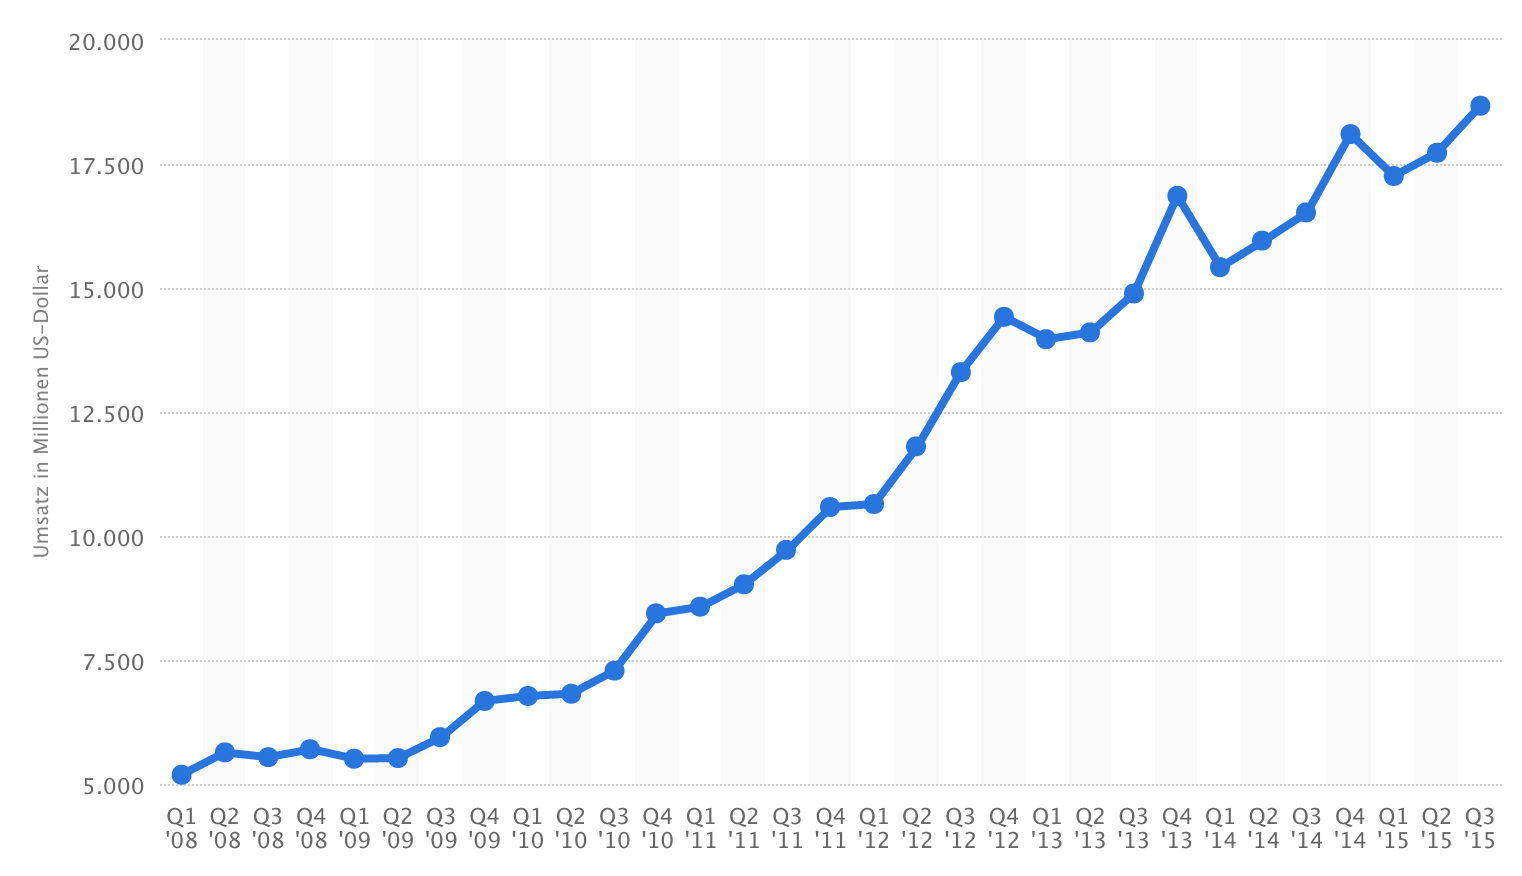
\includegraphics[width=0.9\textwidth]{../graphics/images/google_revenue.png}
	\caption{Revenue of Google in Mio. USD, © 2016 Statista, Source: \url{http://de.statista.com/statistik/daten/studie/154635/umfrage/umsatz-von-google-quartalszahlen/}
}
\end{figure}

\subsection{Open Source and Software as a Service (SaS)}
\label{sec:sas}

Many companies are implementing OSS as a part of their software service nowadays. This means, software services are usually offered through a platform (which is the internet by default). The terms \textit{Software as Service (SaS)}, \textit{Cloud Services} and \textit{Cloud Computing} imply that the service is only available via remote rather than installed as local software. Thus, SaS is rather rented than licensed (\cite{buxmann2008software}) and, compared with traditional locally installed software, profit is generated by leasing the software and service to the user.

The range of open and closed source code behind software services differs widely. Server side components and frontend modules often rely on OSS technologies \footnote{for example: many services using OS databases like MariaDB or PostgreSQL for data storage}. Because most SaS-APIs only allow receiving and returning (processed) users' data, those closed server-side processes make studying executed code hard or even impossible. Thus, the user is neither able to determine what the software really does nor able to change (and redistribute) it (\cite{WhatDoesThatServerReallyServe:online}). Therefore, this approach is widely against the initial thoughts of free software.

Moreover, cloud computing aims to force people to buy lock-in systems that will increase costs over time (\cite{CloudComputingIsATrapWarnsGnuFound:online}). To fill the gap of lacking copyleft on SaS, the free software foundation published the GNU Affero GPL in 2007 (\cite{GNUAfferoGeneralPublicLicense:online}) which demands a download link to the source code on hosted services running the affected software.

Beyond closed-source SaS-providers other companies like \textit{GitLab} (\cite{gitlabraises1.5million:online}) or \textit{ownCloud} (\cite{diycorporatecloudwithowncloud:online}) publish their entire server- and client-side software as OS. Profit is generated by providing enterprise editions (\cite{gitlabraises1.5million:online}; \cite{ownCloudServerOrEnterpriseEdition:online}; \cite[p.148]{van2014gitlab}) \footnote{the enterprise edition does not necessarily differ in features rather than then in support features for the service itself} for instance. Other companies publish and maintain specific libraries or components as OS \footnote{for example: facebook initiated React (\cite{reactnativeannouncement:online}) and uses React Native (\cite{reactnative:online}) in multiple production apps (\cite{reactnativegithubreadme:online})}. The latter is common practice for (larger) technology companies like Google, Microsoft, facebook or Amazon.


\subsection{Open Source and Open Innovation}
\label{sec:open_source_and_open_innovation}

OSS can be regarded as process innovation (\cite{bonaccorsi2003open}) with a connection to open innovation. Information to solve a problem can be sticky and opening innovation can help to solve the problem of sticky information (\cite{von1994sticky}). Open Innovation implies that valuable ideas may come from the inside or outside of a company \cite[p.43f]{chesbrough2006open} and let to the assumption that exploration and exploitation of internal and external ideas lead to better innovation. Using the term "openness" according to \cite{chesbrough2003logic}, "open innovation is a paradigm that assumes that firms can and should use external ideas as well as internal ideas, and internal and external paths to market, as firms look to advance their technology". Thus, companies can turn (technology regarded) ideas from inside and outside the company to profit (\cite{dahlander2010open}).

For the need of companies to connect "Open Innovation" with "Open Source",  \cite{dahlander2010open} give the following reasons:

\begin{itemize}
  \item Social and economic changes in working patterns:
	\begin{itemize}
		\item today employees are seeking more often portfolio careers than a single employer for lifetime
		\item OS commitment builds a better portfolio
	\end{itemize}
  \item Globalization:
	\begin{itemize}
		\item allows increasing division of labor
		\item enables working on distributed channels on source code
	\end{itemize}
  \item Intellectual property rights (IPR), venture capital (VC) and technology standards allow for organization to trade ideas
  \item Software and technology:
	\begin{itemize}
		\item changes the minimum efficient scale of production
		\item allows new ways to collaborate
		\item coordinates across geographical distances
	\end{itemize}
\end{itemize}

As follows, \textit{Open Source} and \textit{Open Innovation} are related terms since programming is a kind of innovation by creating new products (software) to solve (technical) problems.

\subsection{Open Source Collaboration of Firms with external Developers}

As stated in chapter \ref{sec:open_source_and_open_innovation}, OS developers are innovating users (\cite{von2005democratizing}): they evaluate, change and improve source code for their own purpose and solve problems by creating software for specific use cases. Usually they publish their innovations without claiming intellectual property rights and are driven by extrinsic and intrinsic motivation (\cite{hertel2003motivation}; \cite{hars2001working}; \cite{lakhani2002boston}).

Firms' investment in OS software and communities differs from the interest of (external) OS developers since firms expect a return of investment. Their intention of investment is mainly driven by economic, technical and strategic reasons (\cite{wichmann2002free}; \cite{henkel2006selective}). If firms acting in OS sections, conflicts with OS community members may occur due to different interests of contribution (see \cite{IveJustLiberatedMyModules:online} as example), license permissions (\cite{hars2001working}) and commercial intention. Forms of commitment by firms can be participating in software development, communication channels or in general by creating network effects through an "architecture of participation" \cite[p.22]{o2007web}.

But why do firms initiate OS projects and do maintain them even if they do not belong to their core business?

West and Gallagher identified the following benefits when organizations do sponsor OS projects \cite[p.13]{west2006challenges}:

\begin{itemize}
	\item helping to establish their technology as de facto standards (reduces the likelihood of having to re-implement other products to conform to competing standards)
	\item attracting improvements and complements that make the technology more attractive
	\item together, the innovation and complements enable the sale of related products
	\item generating mindshare and goodwill with the same audience that includes the potential
customers for these related products
\end{itemize}

As \cite{tsay2014influence} found out, contributions on GitHub by submitters with high status in the community and a stronger social connection to the project have a higher chance to get accepted. Besides, discussions of contributions have a social and technological factor. Contributions on established projects are harder to be accepted (\cite{tsay2014influence}) which may occur trough higher communication costs. In addition, employed developers who work for longer periods on firms' initiated OS projects have a higher reputation in the community, more power of control on contributions and larger influence of project's (technical) design and advancement.

Consequently, firms may receive indirect (nonmonetary) return of investments if they initiate and maintain projects that are not primary relevant for (monetary) revenue. Better reputation and establishment of software technology with more success are such returns as well as coming across new potential employees \footnote{external developers are potential employees since they have project related knowledge and matching skills}.

\subsection{GitHub as Host for observed Projects}

GitHub is the largest social coding repository and hosts over 35 Mio. repositories by 14 Mio. people (\cite{AboutGitHubPress:online}; \cite{HowGitHubConqueredGoogleMicrosoftAndEveryoneElse:online}). It was successfully used as data source in several other studies before (\cite{vasilescu2013stackoverflow}; \cite{tarrell2016GenderBiasInOpenSource}; \cite{dabbish2012social}; \cite{thung2013network}) and allows to query project related metadata. Moreover, all popular firms do publish their OS projects mainly on GitHub because it offers extended enterprise support (\cite{IntroducingGitHubEnterprise:online}) \footnote{against payment of a fee, \url{https://enterprise.github.com/features}} beside it's popularity for free and public accessible projects.

\subsection{Increasing commitment of Companies to Open Source}

\subsubsection{As an example of developing a common approach: Microsoft and Open Source}

Between the late 90s and the beginning of the century Microsoft was widely known for it's rigorous distaste towards OS licenses, OSS and especially the \textit{GNU/Linux} system. At this time Microsoft's core product and cash cow was Microsoft's operating system Windows (\textit{MS Windows} for clients \& \textit{MS Windows Server}) and \textit{Microsoft Office} \cite[p.2]{reifman2007microsoft}. In other words, Microsoft got threatened by OSS. This was regarding particular Linux as client and server operating system and \textit{OpenOffice} (nowadays widely known as fork \textit{LibreOffice}). This may be one of the reasons why former Microsoft CEO \textit{Steve Ballmer} regards \textit{Linux} (and it's GPL license) in 2001 as cancer that attaches itself in an intellectual property sense to everything it touches (\cite{ballmerlinuxcancer:online}).

Since user interaction with the operating system shifted from local machines (i.e. locally installed software on stationary computers) to the internet (using software services in the web browser and on mobile devices, as described in chapter \ref{sec:sas}), Microsoft couldn't defend its dominant position and lost market shares in the last decade (\cite{MicrosoftWindowsOEMandOfficeRevenueIsDownAsCloudGrows:online}).

By failing to defend the dominant position of their proprietary software, \textit{Microsoft} started to change their strategy over the last decade and increased their commitment in OSS. As \textit{Sam Ramji} already stated in 2008 (\cite{microsoftosstrategy2008:online}), \textit{Microsoft} has realized to include \textit{Linux} (i.e. other OSS and OS based services) as a vertical product integration in a heterogeneous environment on top of \textit{Windows}. This strategy of mixing OSS with proprietary software (\cite{mixingosandproprietarysoftware:online}) is common practice in technology companies nowadays.

In 2014 \textit{Microsoft} announced to publish their programming language and enterprise framework \textit{.NET} as open source (\cite{msnet2015os:online}). This step was just one of their latest upcoming OS commitments and facing towards the OS community (see \cite{microsoftchakracoreonline:online} as one of the latest examples).

Finally, \textit{Microsoft} moved in 2015 most of its OS projects from codeplex (their own OS hosting service) to \textit{GitHub} (\cite{msmovingtogithub2015:online}). With this step \textit{Microsoft} tries to reach the vibrant OS community (of \textit{GitHub}) and indicates that they want to be an active part of it. Currently, Microsoft's GitHub account contains more than 370 projects with 1,138 organizational developer profiles (external developers are excluded) \footnote{Retrieved \nth{9} January 2016}.

\subsubsection{GitHub's Atom Editor and Microsoft's Visual Studio Code as example for technology exchange between firms and collaboration with the OS community}

In 2011 \textit{GitHub Inc.} \footnote{to "distinguish" between the company and the community, we will use \textit{GitHub Inc.} for the company; but the transition is seamless sometimes} employee \textit{Corey Johnson} and \textit{GitHub} founder \textit{Chris Wanstrath} started building the \textit{Atom editor} (hereafter referred to as \textit{Atom}) as closed source project inside the \textit{GitHub} company (\cite{AtomV1:online}). \textit{GitHub} conceived the \textit{Atom} in February 2014 to the public (\cite{IntroducingAtom:online}). In May 2015 they published its source code (\cite{AtomIsNowOpenSource:online}) under the \textit{MIT License}. The idea of the \textit{Atom} is to be a "zero-compromise combination of hackability and usability" and therefore a rival software product to other closed source / commercial editors like \textit{Sublime}, \textit{Apple's XCode} and \textit{Microsoft's Visual Studio}. The feedback of the OS community was widely positive and \textit{Atom} gained quickly considerable attention  (\cite{AtomIsJustGettingStarted:online} and \cite{AtomReachesOneMillionActiveUsers:online}).

One key feature of \textit{Atom} is its modularity, which allows customization through "packages" (i.e. "plugins"). Each plugin is customized for specific software development needs. The format of packages and themes was previously introduced by \textit{Sublime}, which holds a large repository of plugins. Thus, all \textit{Sublime} plugins can easily be converted to \textit{Atom}
\footnote{\url{https://discuss.atom.io/t/convert-sublime-grammar-to-atom-grammar/14843}}.
In addition, the introduction of \textit{apm} (\textit{Atom Package Manager} \footnote{\url{https://github.com/atom/apm}} as central software provider for those plugins enabled a new software ecosystem for the editor and accelerated the acceptance of converting, building and deploying new plugins for \textit{Atom} by the community.

\begin{table}[!h]
\centering
\begin{tabular}{rlllll}
  \hline
 & Themes & Packages & Users & Authors & Downloads \\
  \hline
Atom & 1,008 & 3,496 & - & - & 32,79M \\
  Sublime & 295 & 3,426 & 4,6M & 2,477 & - \\
   \hline
\end{tabular}
\caption[Available Plugins for Atom Editor and Sublime Editor]{Available Plugins for \textit{Atom Editor} and \textit{Sublime Editor}; Retrieved on: \nth{21} January 2016 \protect\footnotemark}
\label{tbl:atomsublimeplugins}
\end{table}

\footnotetext{\ \ Source: \url{https://atom.io/packages}, \url{https://packagecontrol.io/stats}, \url{http://colorsublime.com}}

A year after the initial release of \textit{Atom}, \textit{Microsoft} announced its free and open source editor \textit{Visual Studio Code} (\textit{VSC}) (\cite{MicrosoftLaunchesVisualStudioCode:online}). \textit{VSC} is a code editor with similar look-and-feel, features and ideas of \textit{Atom}, but initiated by \textit{Microsoft}. Moreover, \textit{VSC} is based on \textit{Electron} (\cite{electroncrossplatformapps:online}) and \textit{React} - both are OS technologies by \textit{GitHub Inc.} and \textit{facebook} respectively and core technologies of  \textit{Atom} as well.

This makes \textit{VSC} to a rival product with the potential to substitute \textit{Atom}. Using \textit{Electron} and some other core libraries as foundation, \textit{VSC} guarantees interoperability of \textit{Atom's} plugins on its editor. In November 2015 \textit{Microsoft} finally published \textit{VSC} as open source likewise  (\cite{VSCodeIsOpenSource:online}).

\textit{GitHub Inc.} and \textit{Microsoft} are aware that the editor gets only established with a variety of plugins (see table \ref{tbl:dataofvscodeandatom}) and with an active community. The reason is that establishing software standards is to some degree a Winner-Take-All market. Once a standard is established in the community (here an editor with a specific API and package format) the development of "plugins" will be successful, too.

This example demonstrates how two firms published initially closed source developed software as open source: \textit{Atom} (\textit{GitHub Inc.}) and \textit{VSCode} (\textit{Microsoft}). Both editors are heavily using OS libraries as technical foundation.

Altogether, Microsoft's editor is a good example of

\begin{itemize}
	\item using OS technology of competitors (\textit{GitHub Inc.}, \textit{facebook} and \textit{Instagram})
	\item as foundation to build OSS for the community
	\item with plugins and code contribution by the community and developers by competitors
\end{itemize}

\textbf{Interpretation:} The reason why both firms decided to publish their projects as open source may be that the OS developers are their target customers (\cite{IntroducingAtom:online}), community members and potential employees. By providing technologies for the community, both firms will improve their reputation in the developer community. Furthermore, upcoming projects will be easier accepted by external developers, more likely successful and establishing software technology in future might be more feasible in a smaller amount of time.

\textit{A further analysis of "Atom" and "VSC" ("Microsoft" and "GitHub Inc." respectively) can be found in chapter \ref{sec:atom_vs_vsc} on page \pageref{sec:atom_vs_vsc}}

\clearpage
\subsection{Forms of Participation on GitHub Projects}
\label{sec:forms_of_participation_on_github}

\begin{figure}[!h]
	\centering
	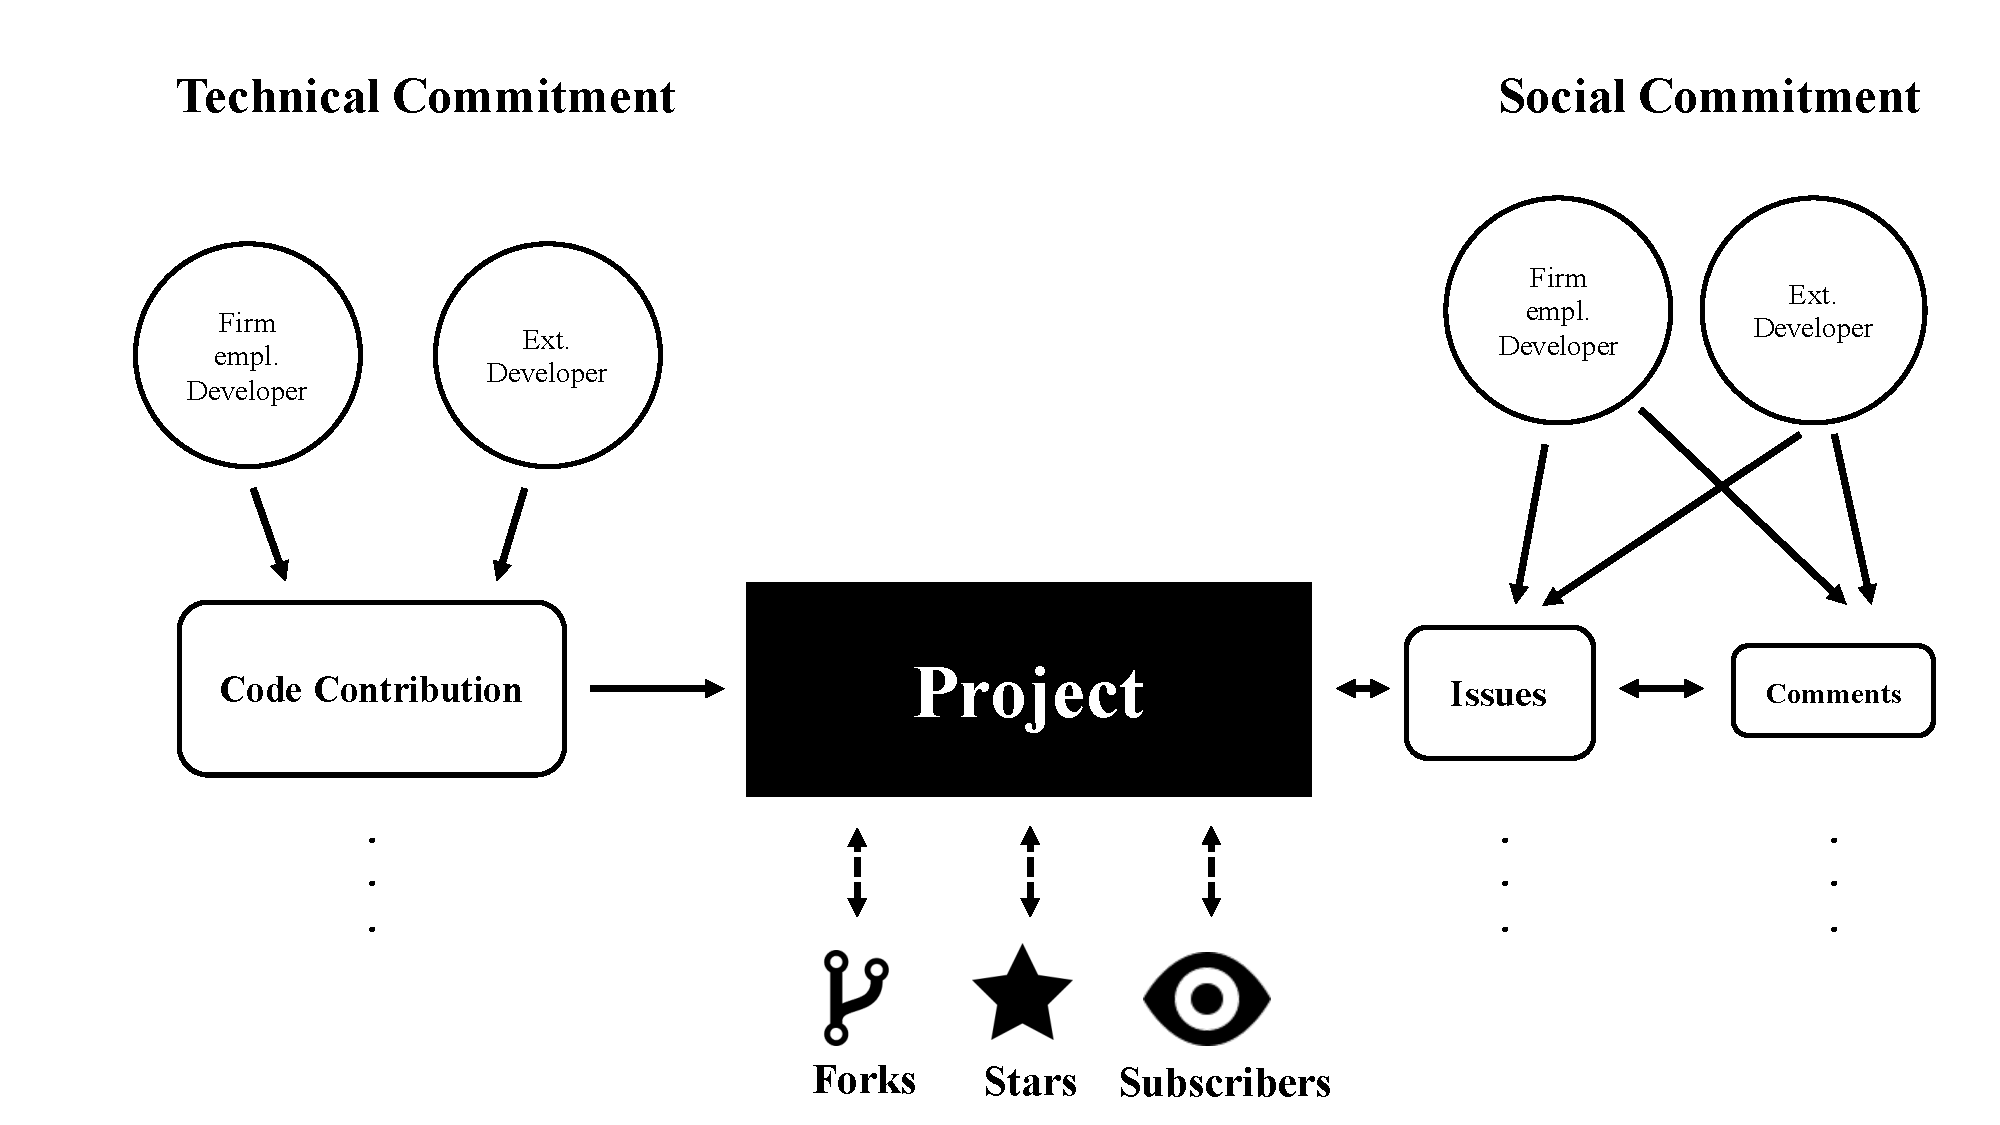
\includegraphics[page=1,scale=0.45]{../graphics/figure_contribution.pdf}
	\caption{Technical and social Commitment in GitHub Projects}
	\label{fig:forms_of_commitment}
\end{figure}

GitHub allows direct and indirect participation. This implies that every user can participate with minimum action (indirect) and active contribution (direct).

The following technical and social participations are possible:

\begin{itemize}
	\item Code Contribution (direct)
	\item Creating Issues (direct)
	\item Participation by commenting on Issues (direct)
	\item \textit{Fork}, \textit{Subscribe} and \textit{Star} project (indirect)
\end{itemize}

Use and interpretation of these attributes will be explained in chapter \ref{sec:social-success-metrics} on page \pageref{sec:social-success-metrics}.

\clearpage
\subsection{Linear and Logistic Regression Models}

The empirical analysis uses \textit{Linear \& Logistic Regression Models}. According to Seber and Lee we can describe the linear models of the study as follows \cite[p.35]{seber2012linear}:

\begin{align}
	 \text{lm}_{j} &: y_{\text{j}_{i}} &= \beta_{j_{0}} + \beta_{j_{i}} x_{j_{i}} + \dots + \varepsilon_{j_{i}} \\
	 & & x : \textit{explanatory variable} \nonumber \\
	 & & \varepsilon : \textit{fluctuation} \text{ or } \textit{error} \nonumber \\
	 & & \beta : \textit{unknown parameter} \nonumber \\
	 & & \text{lm} : \textit{linear model} \nonumber \\
	 & & \forall i \in \textit{observations} \nonumber \\
	 & & \forall j \in \textit{linear regression models} \nonumber
\end{align}

The independent and dependent variables will be different regarding to model assumptions. In particular \textit{Ratio} (share of contribution by internal developers) and \textit{Age} will be set as independent variable, \textit{share of contribution by external developers} and \textit{Top Project} set as dependent variable. \textit{Firms} and \textit{Programming Languages} will be used as dummy variables in some models.

Because \textit{Top Project} is $\in \{0, 1\}$, the \textit{logit model} is used in this case \cite[p.23]{hilbe2009logistic}:

\begin{align}
	 \mu_{j_{i}} = \frac{ 1 }{ 1 + e^{-x_{j_{i}} \beta_{j_i}} } \\
	 & & \mu : \textit{fitted value} \nonumber \\
	 & & \forall i \in \textit{observations} \nonumber \\
	 & & \forall j \in \textit{logistic regression models} \nonumber
\end{align}

\subsection{Fitting Linear Mixed-Effects Models}

To consider effects within \textit{Firms} and effects within \textit{Programming Languages} some analyses will be handled additionally by \textit{Fitting Linear Mixed-Effects Models} \cite[p.13]{R_lme4}: \footnote{as mentioned in \cite[p.1]{R_lme4}, "mixed effects" denotes a model that incorporates both fixed- and random-effects terms}

\begin{align}
	\eta_{j} = X\beta_{j} + Z\gamma_{j} + \varepsilon_{j} \\
	& & \eta : \textit{known vector} \nonumber \\
	& & \gamma : \textit{unknown vector of random effects} \nonumber \\
	& & \beta : \textit{unknown vector of fixed effects} \nonumber \\
	& & \varepsilon : \textit{unknown vector of random errors} \nonumber \\
	& & \forall j \in \textit{linear mixed-effects models} \nonumber
\end{align}

\clearpage
\subsection{Hypotheses}
\label{sec:hypotheses}

Derived from motivation, theory and previous studies \footnote{\cite{hill2009idea}; \cite{dahlander2014open}; \cite{piezunka2013study}; \cite{dahlander2005relationships}; \cite{alexy2012managing}; \cite{tsay2014influence}; \cite{west2006challenges}; \cite{krishnamurthy2016peripheral}} we formulate the following hypotheses:

\begin{itemize}
    \item [\textbf{H 1}] Firm employees' participation affects the participation of external developers
		\begin{itemize}
			\item [\textbf{H 1.1}] If firm employees contribute source code more often, external developers do as well
			\item [\textbf{H 1.2}] If firm employees participate more often on issue threads, external developers do as well
		\end{itemize}
    \item [\textbf{H 2}] Firm employees' participation (in the beginning) affects the (later) success of firm-initiated open source projects
		\begin{itemize}
			\item [\textbf{H 2.1}] If firm employees contribute source code more often in the beginning, the project gets more successful
		\end{itemize}
		\item [\textbf{H 3}] If firm employees' contribution share is higher overall the more likely the project is popular
\end{itemize}


The analysis will contain code contribution (technical commitment) and participation on issues and comments on issues (social commitment) \footnote{whereby issue participation can also be technical in some cases}. Contribution will be measured with a "standardized contribution share" in respect of (social) success metrics and relations between firm employed developers and external developers. All hypotheses will be verified with firms' publicly available OS projects on GitHub.
